% ------------------------------------------------------------------------------
% section 02
% ------------------------------------------------------------------------------
\newpage
\section{Questions 2} 
\label{cha:q2}

\subsection[Q2-a]{Create a new data frame only including "Airbus $A320$", "Airbus $A350$", "Boeing 737" and "Boeing 777" models of airplanes. Check the distribution of Price: first for the observations in this sample and then for each model in the data frame. Interpret your findings.}

\begin{figure}[htbp]
    \centering
    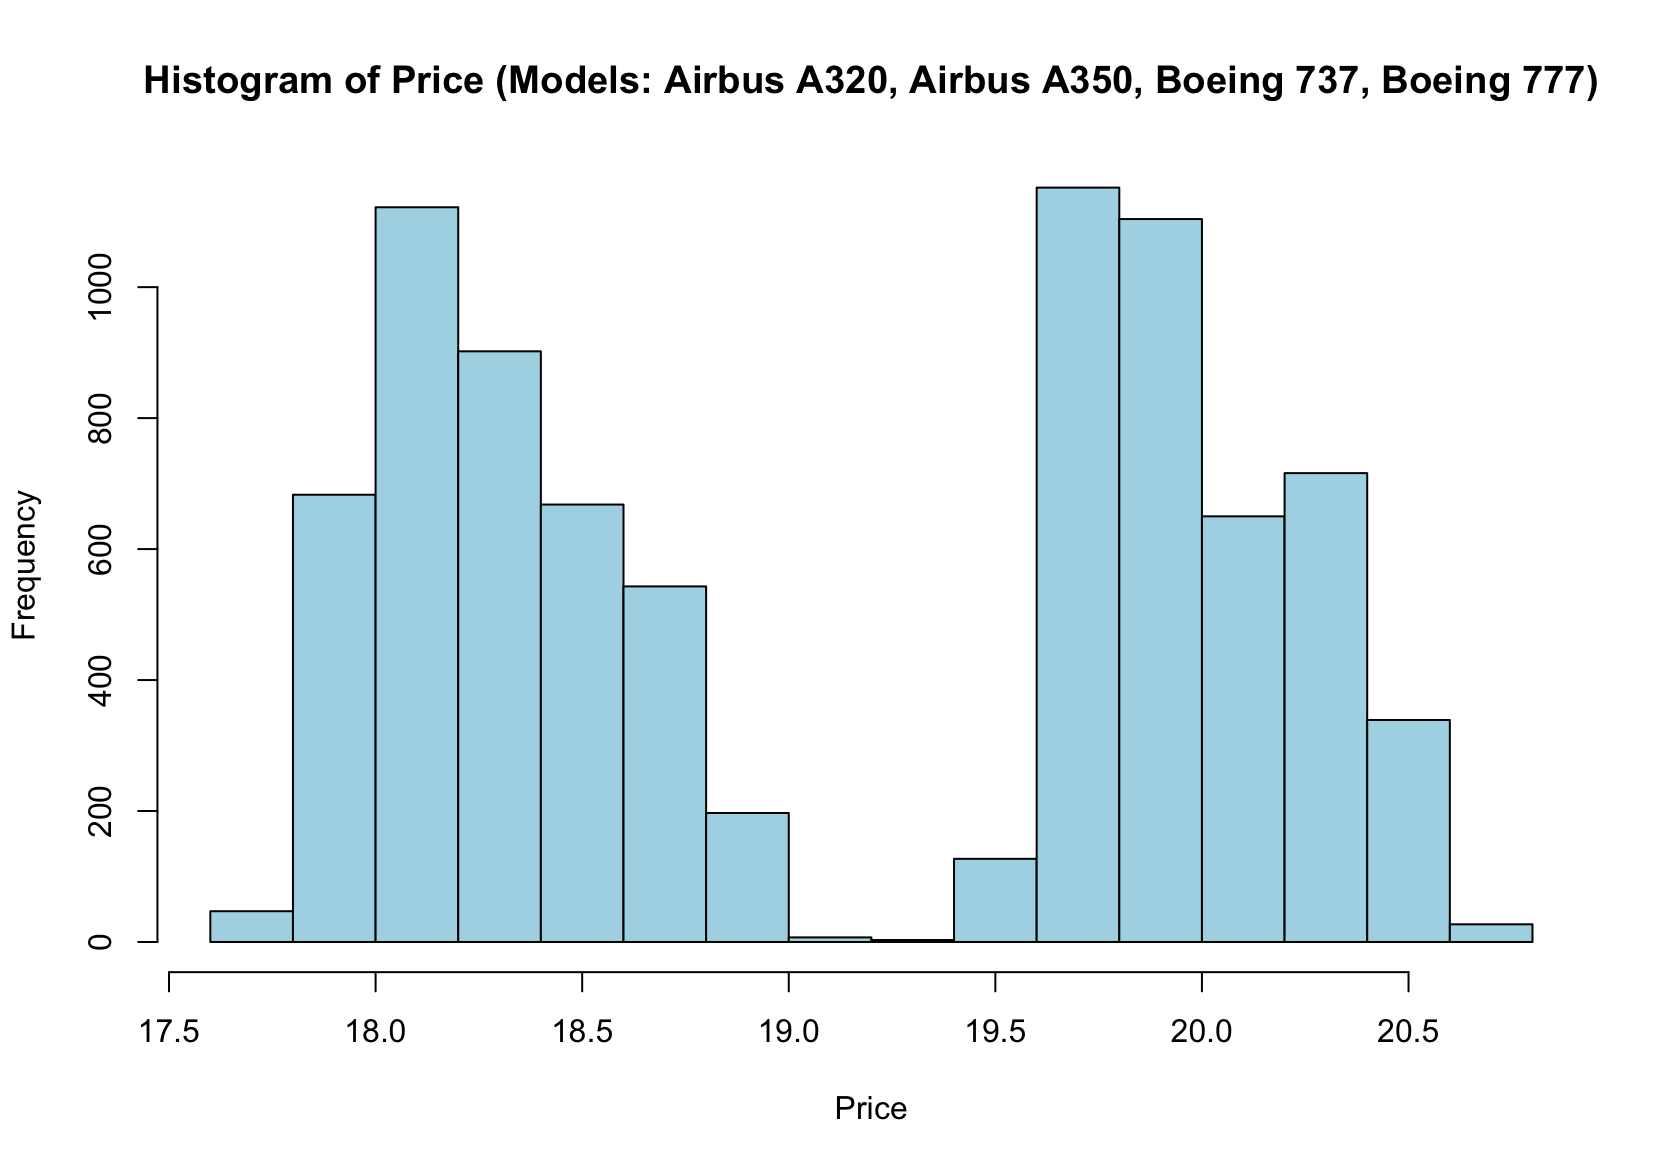
\includegraphics[width=\figsizetext]{Q2/01-summary-price-all.png}
    \caption{Price for all selected models}
    \label{fig:01}
\end{figure}

After the log transformation, Price is approximately normally distributed overall. Per model, Boeing 777 and Airbus $A350$ have higher mean $\log(\text{Price})$ values reflecting their larger capacity and longer range. Boeing 737 and Airbus $A320$ cluster at lower price levels. Within each model, the $\log(\text{Price})$ distribution is roughly symmetric, confirming that log transformation was appropriate for subsubsequent ANOVA analysis.

\begin{figure}[htbp]
    \centering
    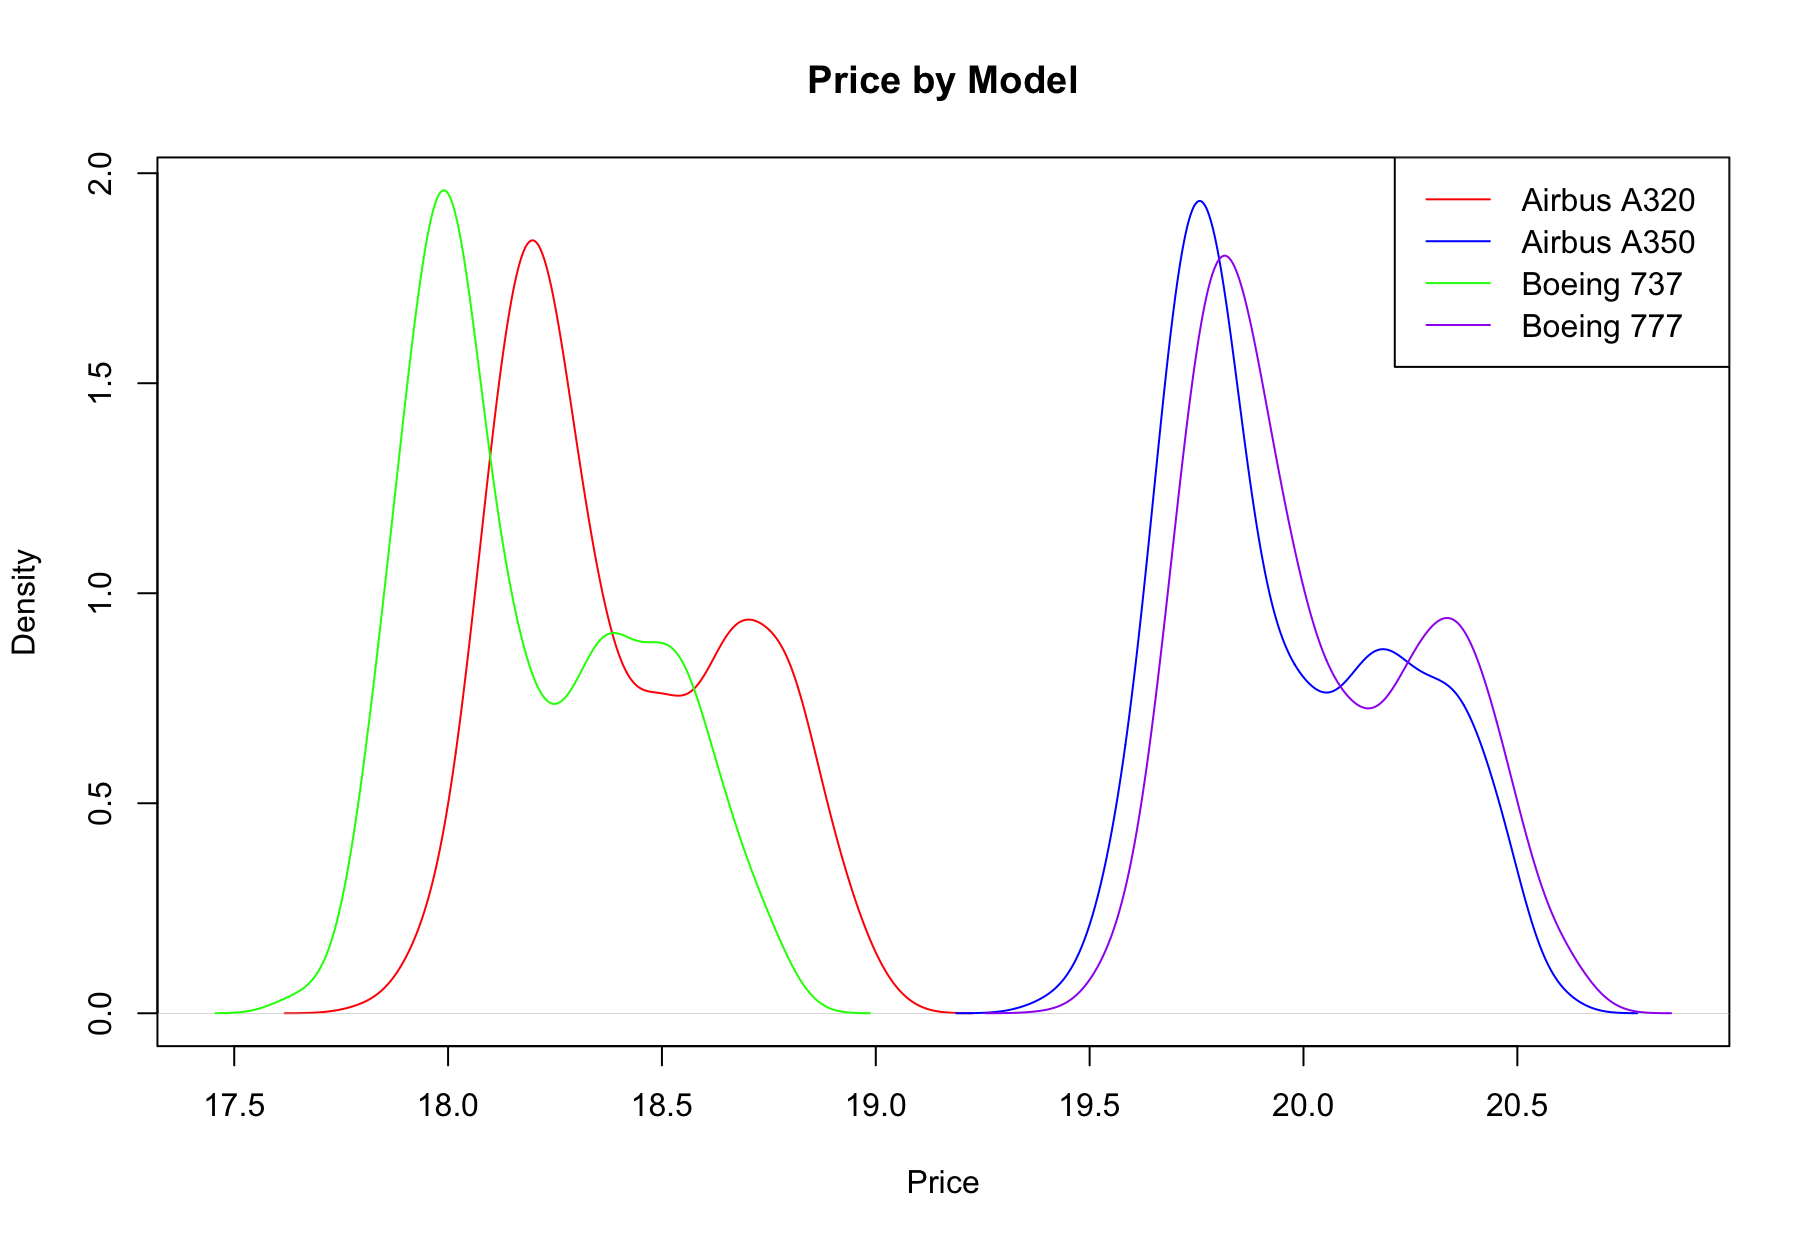
\includegraphics[width=\figsizetext]{Q2/02-summary-price-by-model.png}
    \caption{Price by model}
    \label{fig:02}
\end{figure}

\subsection[Q2-b]{Analyze the numerical variables that are affected by the "Model". Test the assumptions of the statistical method, for the cases that you have found a significant association, by using corresponding tests and plots. Write your conclusions.}

We first used a visual approach to filter the variables that had no significance. The boxplots in figure \ref{fig:03} show that the four models fall into two subsub-groups: cheaper and more expensive models. This difference created a change in some variables, but left untouched others. The next subsection highlights our analysis.

\begin{figure}[htbp]
    \centering
    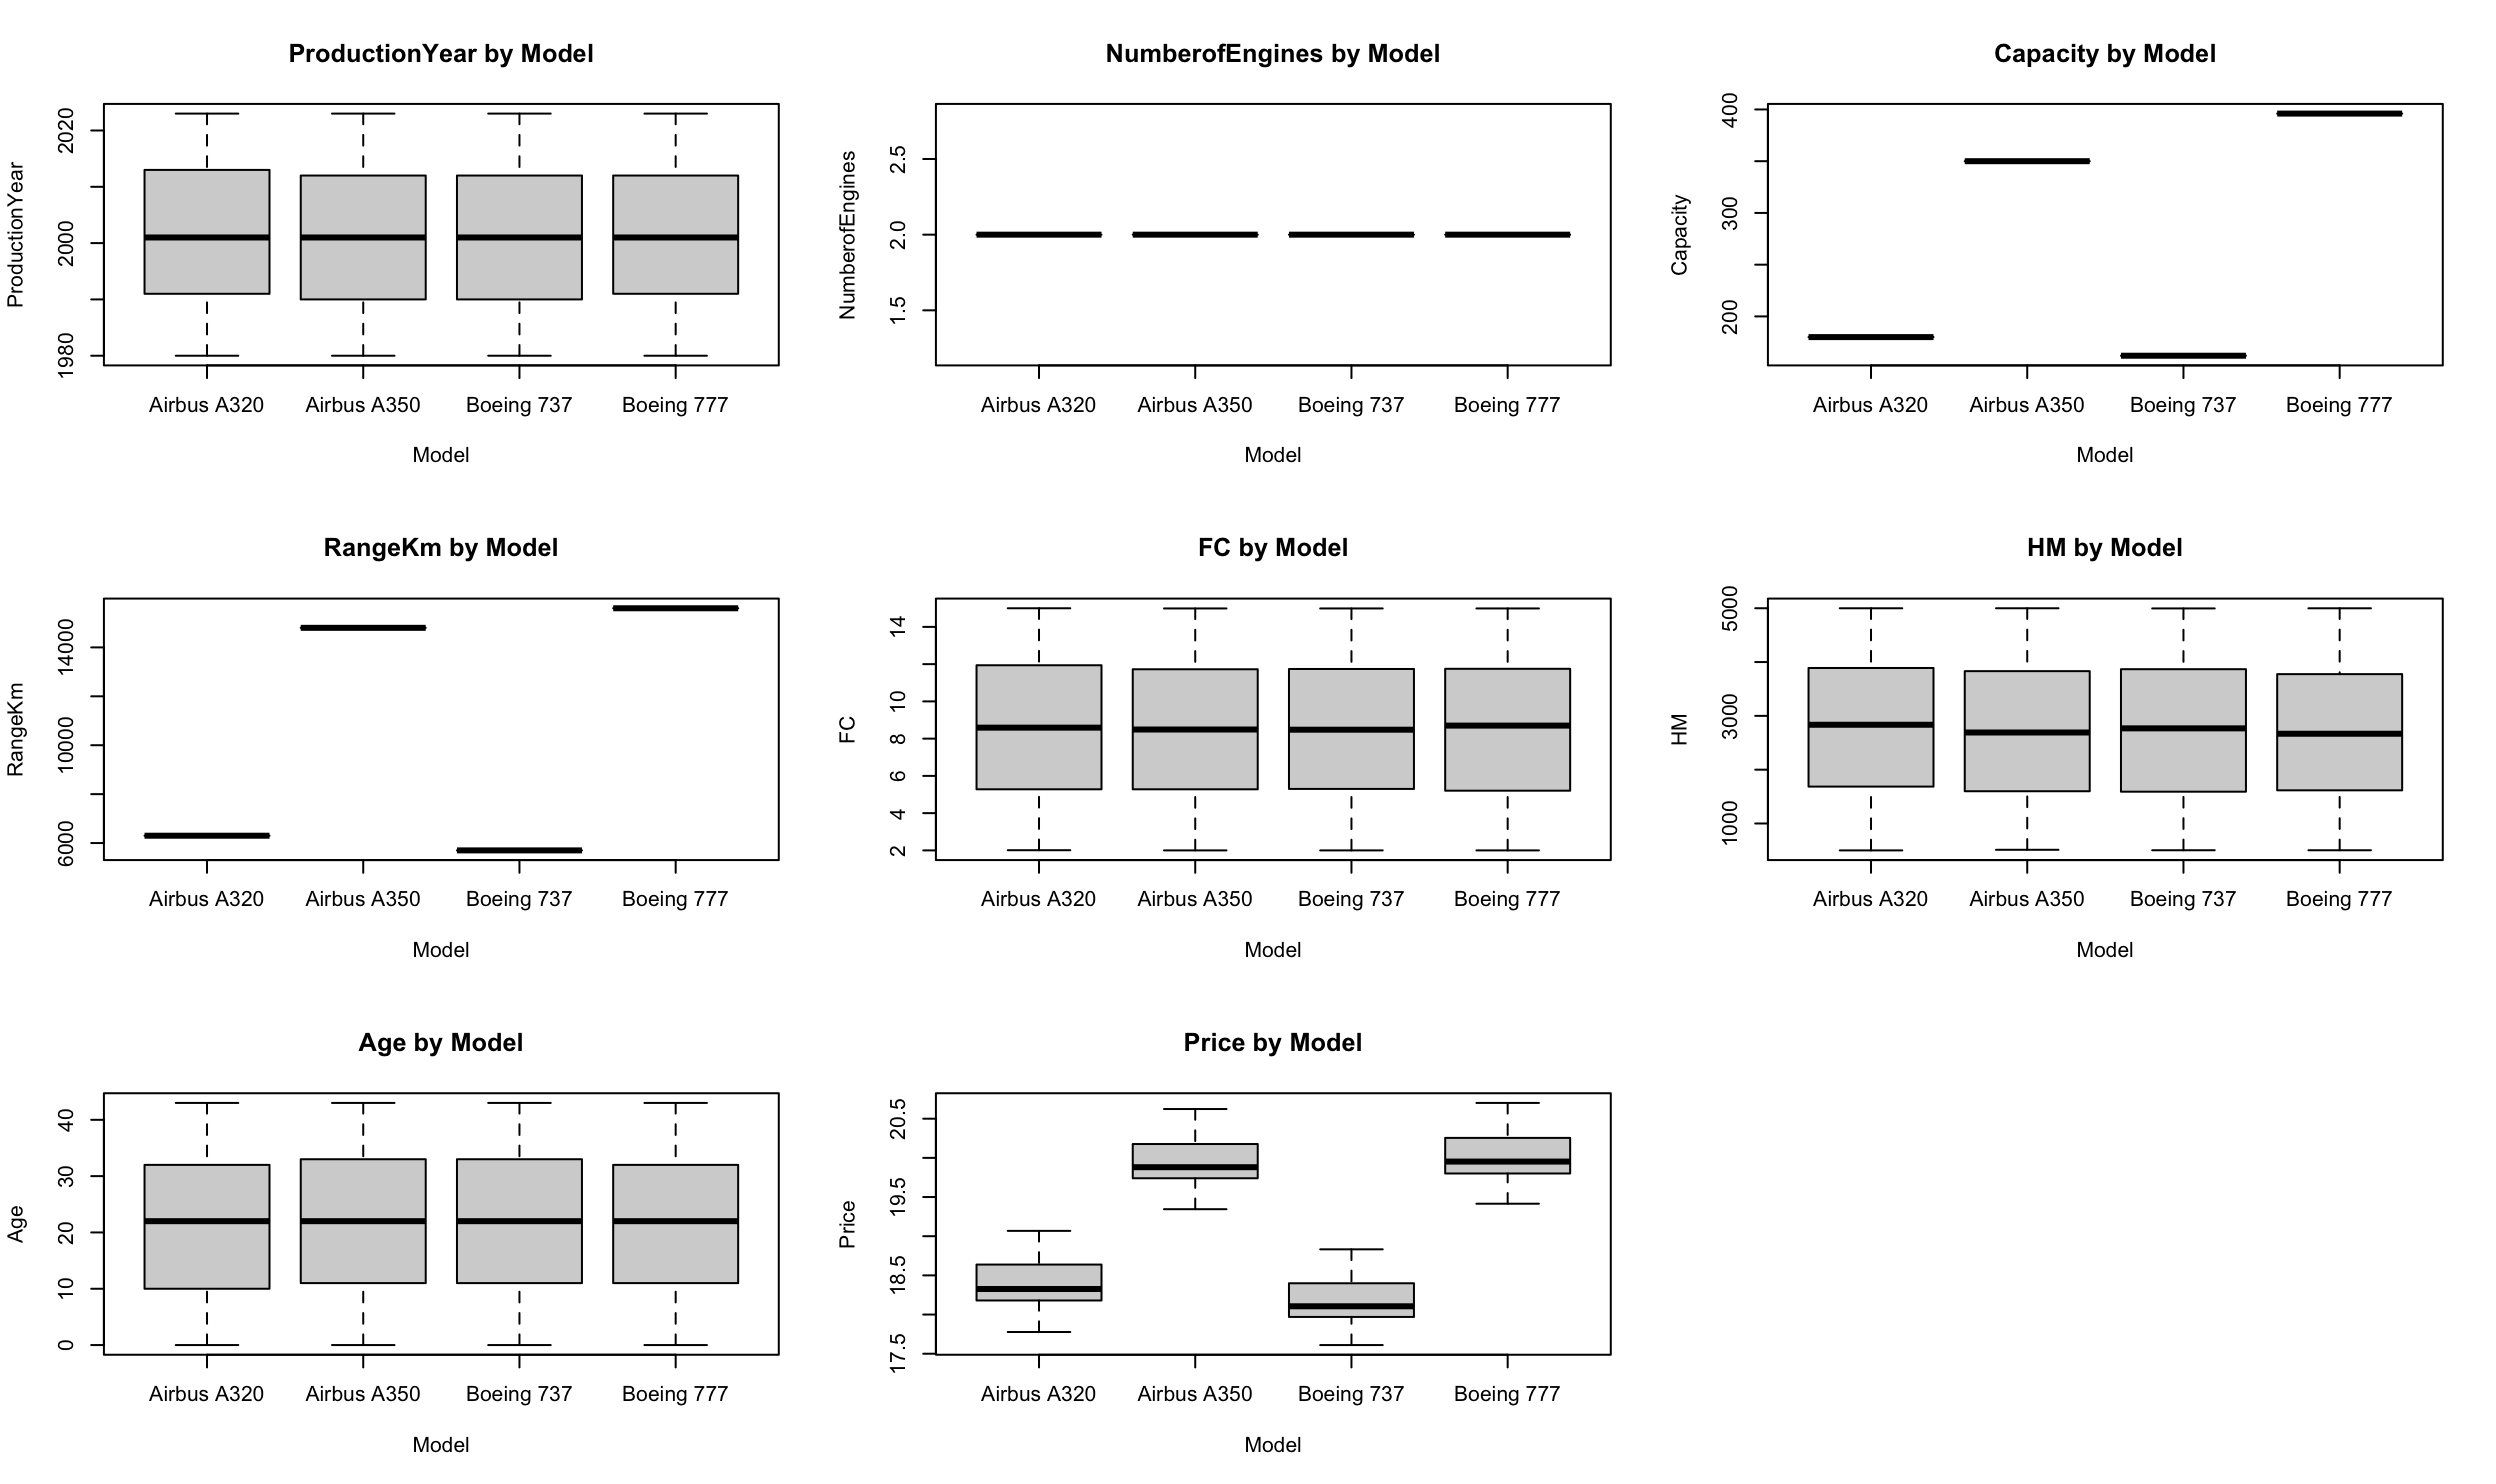
\includegraphics[width=\figsizetext]{Q2/03-boxplot-of-numerics.png}
    \caption{Boxplot of numerical variables}
    \label{fig:03}
\end{figure}

\subsubsection*{Variables Affected by Model}

\begin{itemize}
    \item \textbf{Price}: The $A350$ and $B777$ (expensive subsub-group) are in a different wealth bracket compared to the $A320$ and $B737$ (cheaper subsub-group).
    \item \textbf{Capacity and RangeKm}: These are affected by the model, though there is almost zero variation within groups in the dataset. This means Model, Capacity, and RangeKm are all telling the model the same thing (high multicollinearity).
    \item \textbf{FC, HM, and Age}: NOT significantly different across models since all four are Turbofan jets and the dataset appears to have similar distributions for these.
\end{itemize}

\subsubsection*{Assumption Analysis}

We analyzed only the variable that passed the visula test.

\begin{figure}[htbp]
    \centering
    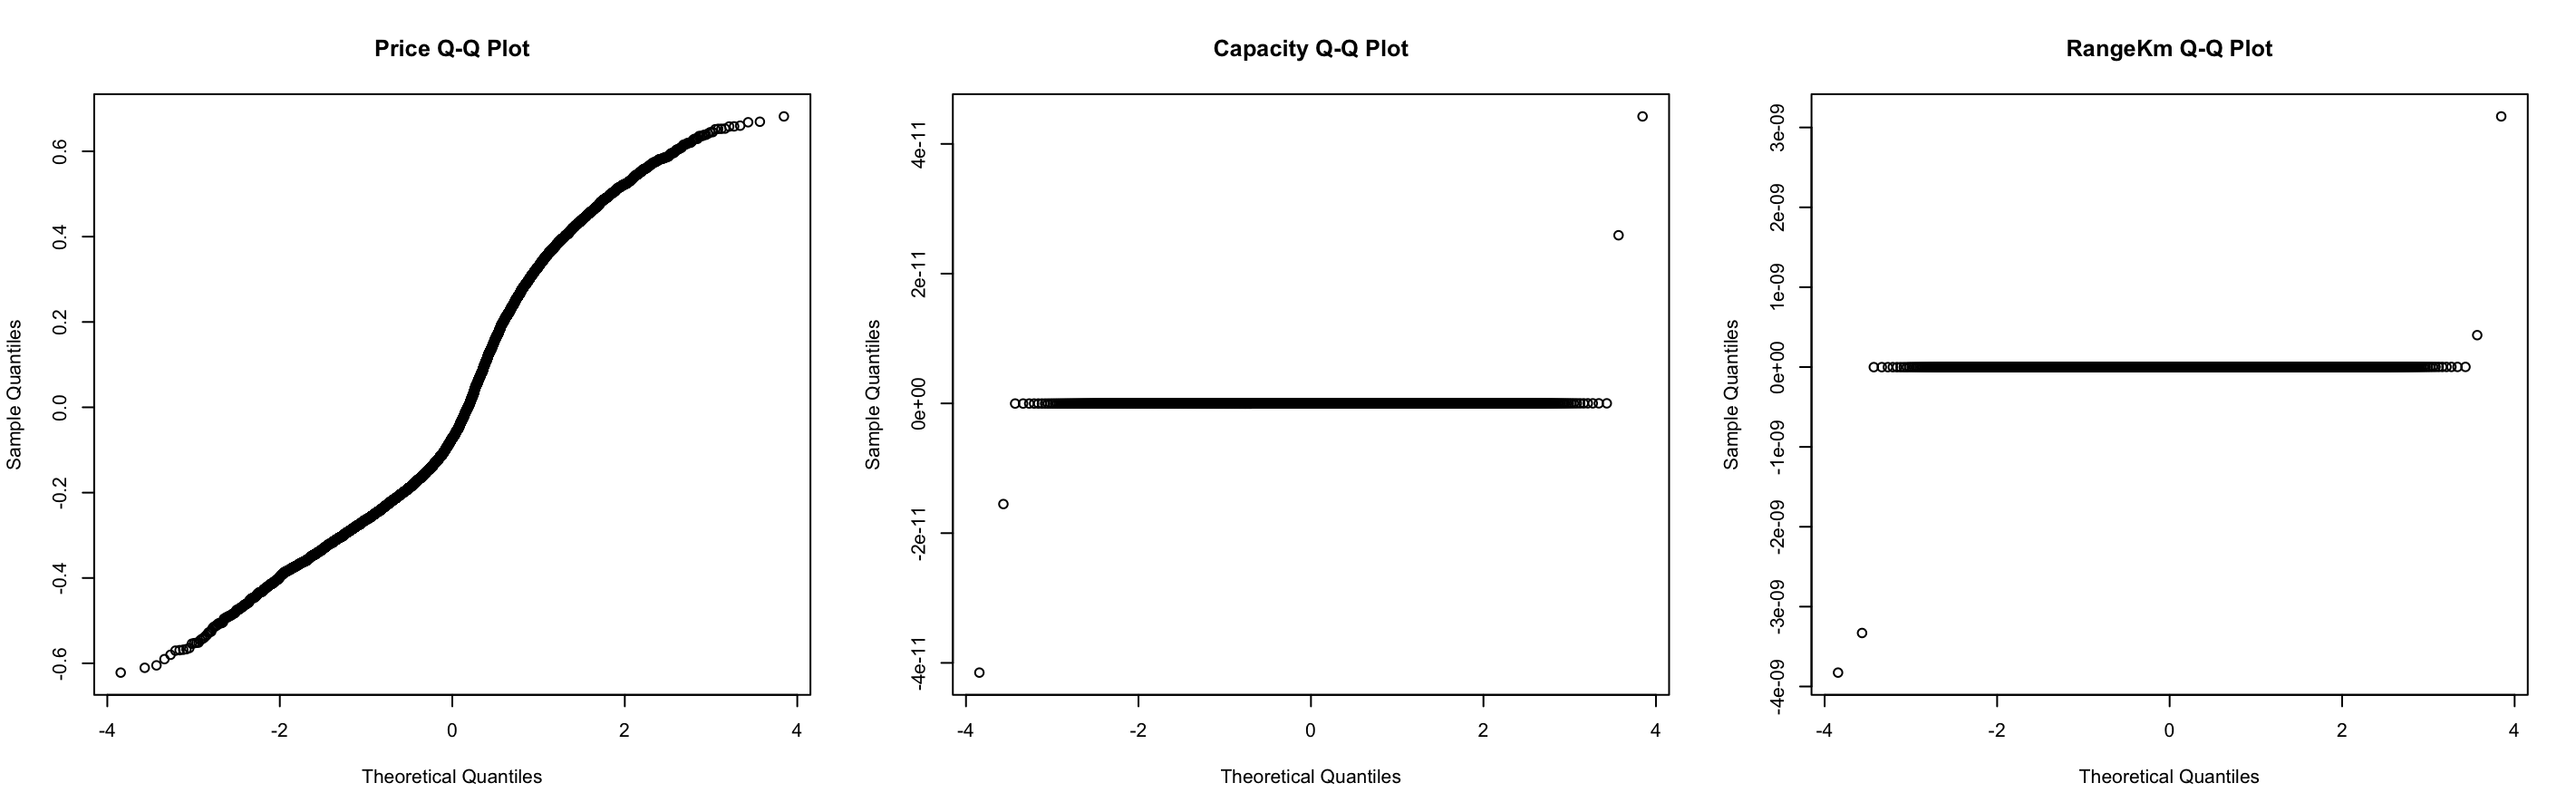
\includegraphics[width=\figsizetext]{Q2/04-qqplot-numerical-all.png}
    \caption{QQ-plot for all numerical variables}
    \label{fig:04}
\end{figure}

\begin{itemize}
    \item The appearance of a "horizontal flat line" in the QQ-plots for \textbf{Capacity} and \textbf{RangeKm} occurs because these are fixed specifications for a given airplane model. Consequently, there is near-zero variance within each model group.
    \item For the case of \textbf{Price} the QQ-plot looks a bit curved with respect to the line meaning it might not be normally distributed. However, both Independence test and Homoscedasticity test show a p-value $> 0.05$ so we are assuming Normality, Independence and Homoscedasticity.
\end{itemize}

\subsubsection*{Conclusion}
The ANOVA p-value for Price is $< 0.05$, so at least one model has a significantly different mean $\log(\text{Price})$. The Tukey HSD test shows which specific pairs differ. We expect $Boeing 777$ and $Airbus A350$ (long-range) to have significantly higher prices than $Boeing 737$ and $Airbus A320$ (medium-range). 

\subsection[Q2-c]{Apply a two-way ANOVA including Sales Region to the model. Interpret your findings.}

We applied ANOVA and the results are reported in table \ref{tab:05}. There is no significant interaction since the p-value is much higher than 0.05, so we can conclude that the relationship between the aircraft Model and its Price does not change based on the Sales Region. Also, while there might be a tiny hint of a regional difference, statistically speaking, Region does not significantly affect Price.

\begin{table}[htbp]
    \centering
    \begin{tabular}{l r r r r l}
        \hline
         & Df & Sum Sq & Mean Sq & F value & Pr($>$F) \\ 
        \hline
        Model             & 3    & 6032 & 2010.7 & 28038.546 & $< 2\text{e-}16$ *** \\
        SalesRegion       & 5    & 1    & 0.2    & 2.142     & 0.0575 . \\
        Model:SalesRegion & 15   & 1    & 0.1    & 0.830     & 0.6445 \\
        Residuals         & 8263 & 593  & 0.1    &           & \\ 
        \hline
    \end{tabular}
    \caption{ANOVA for Price and Region}
    \label{tab:05}
\end{table}

\subsection[Q2-d]{Convert the variable Production Year to a categorical variable with two levels as "Older" and "Newer" and save it as a new variable named "year\_cat" in the data frame.}

To compute the categorization of Production Year we first calculated the median and then applied it to a new variable: $year\_cat$.

\subsection[Q2-e]{Analyze the effect of Model and year ("year\_cat") together on the price. Analyze whether the interaction of two term is significant. Interpret your findings.}

Figure \ref{fig:06} plot aligns with previous analysis: there are two cheaper plane models and two expensive ones, and now we observe that there are older and newer models also which are a bit more expensive (shifted to the right) in each case.
The ANOVA interaction plot shown in figure \ref{fig:08} is just one more analysis that make us sure about what has been deducted before.

\begin{figure}[htbp]
    \centering
    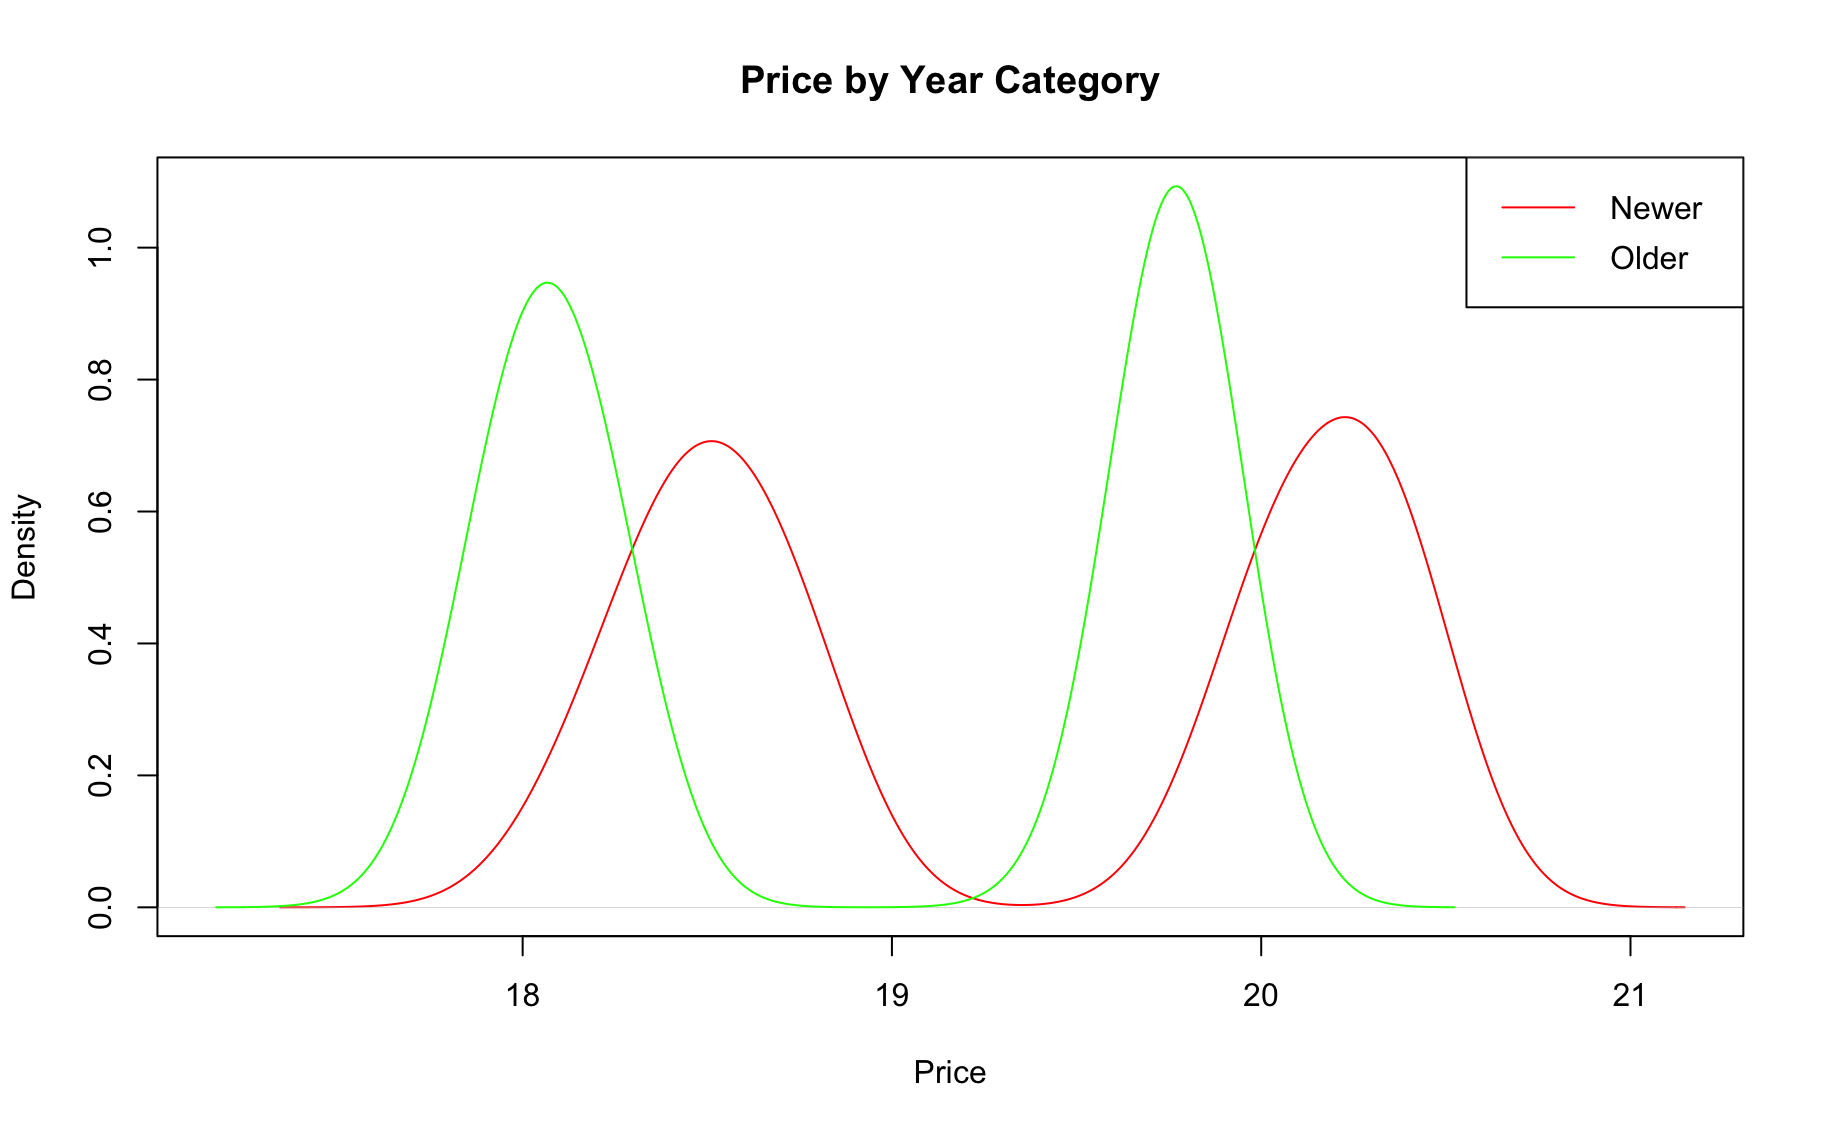
\includegraphics[width=\figsizetext]{Q2/06-plot-by-year-cat.png}
    \caption{Plot by year\_cat}
    \label{fig:06}
\end{figure}


\begin{table}[htbp]
    \centering
    \begin{tabular}{l r r r r l}
        \hline
         & Df & Sum Sq & Mean Sq & F value & Pr($>$F) \\ 
        \hline
        Model           & 3    & 6032 & 2010.7 & 78235.015 & $< 2\text{e-}16$ *** \\
        year\_cat       & 1    & 381  & 381.4  & 14838.647 & $< 2\text{e-}16$ *** \\
        Model:year\_cat & 3    & 0    & 0.0    & 0.984     & 0.399 \\
        Residuals       & 8279 & 213  & 0.0    &           & \\ 
        \hline
    \end{tabular}
    \caption{ANOVA for Price by Model and Year}
    \label{tab:07}
\end{table}

\begin{figure}[htbp]
    \centering
    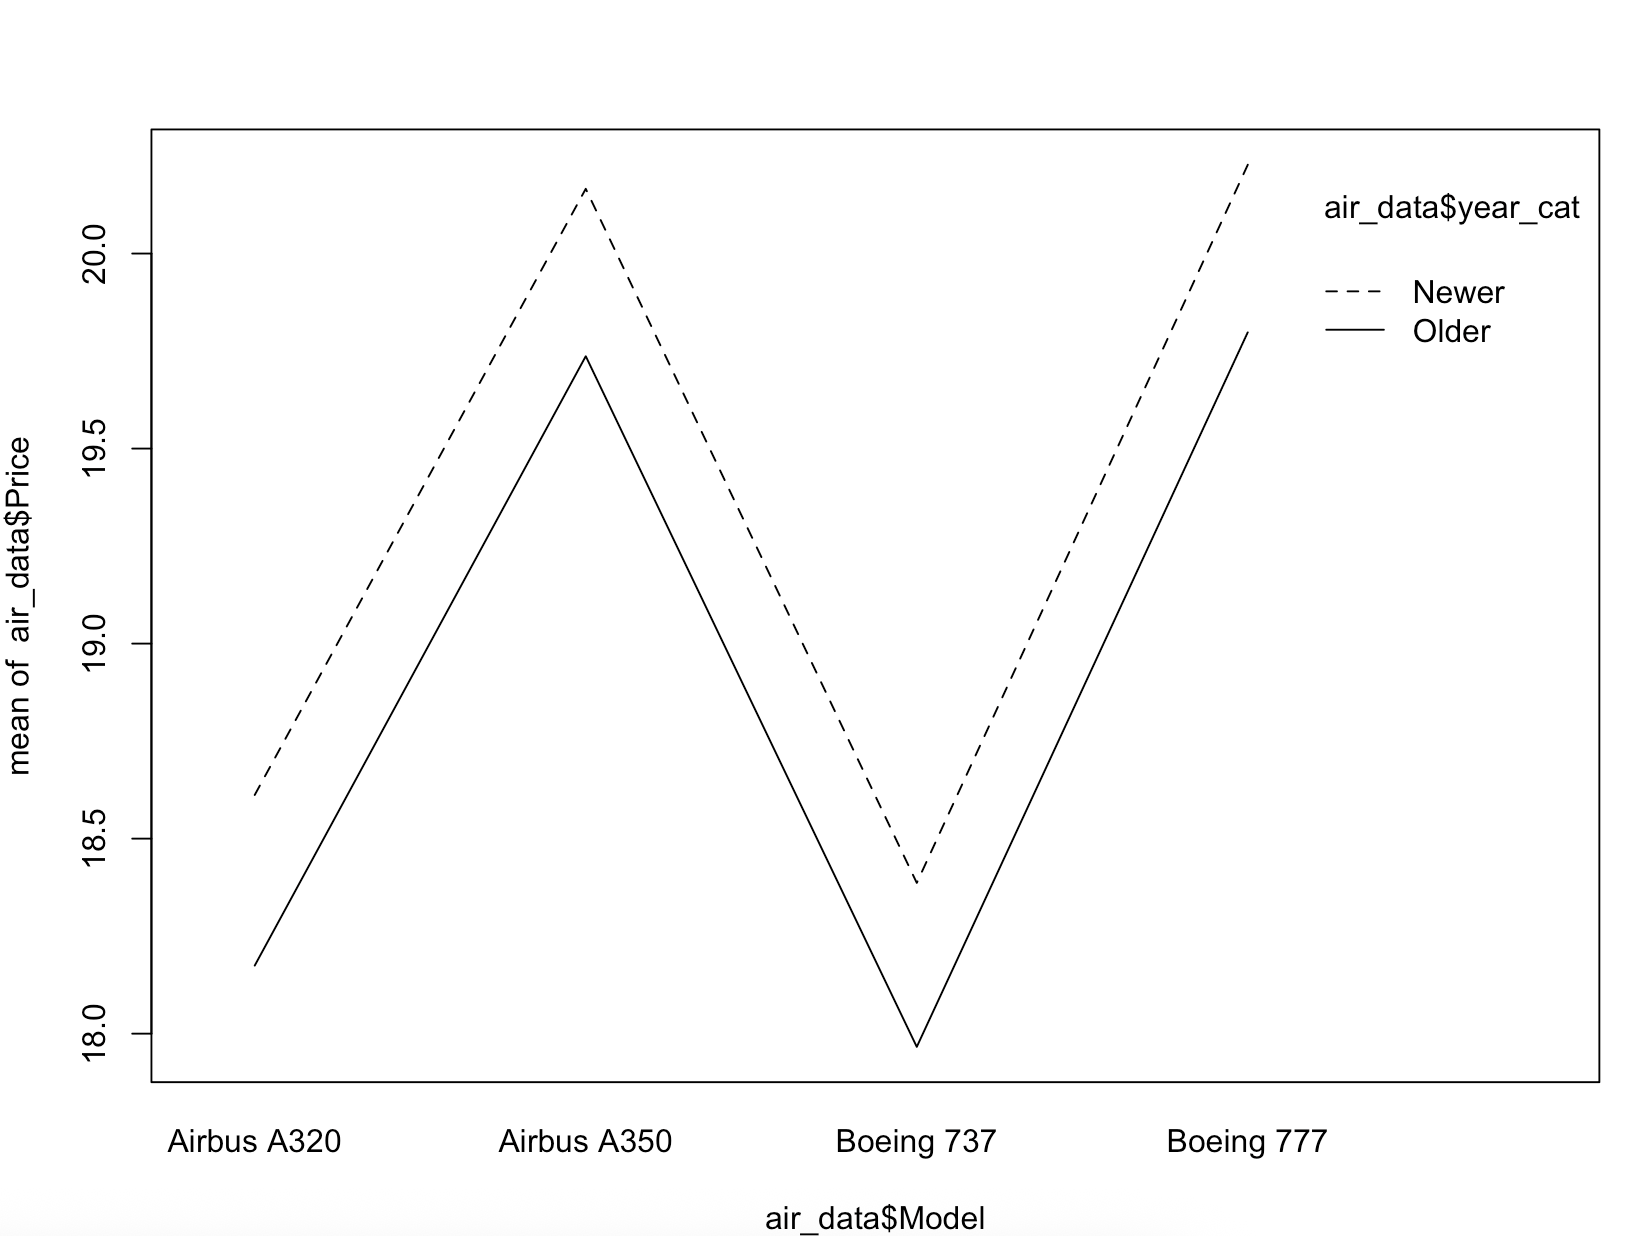
\includegraphics[width=\figsizetext]{Q2/08-anova-interaction-plot.png}
    \caption{ANOVA Interaction Plot}
    \label{fig:08}
\end{figure}

\subsubsection*{Conclusion}

The two-way ANOVA with interaction tests three effects:

%\begin{itemize}
%    \item \textbf{Main effect of Model:} Do different models have different mean prices?
%    \item \textbf{Main effect of year\_cat:} Do newer planes have different prices than older ones?
%    \item \textbf{Interaction (Model:year\_cat):} Does the effect of age on price vary by model?
%\end{itemize}

Based on the two-way ANOVA results, both the airplane Model and the categorized production year (\texttt{year\_cat}) have a significant independent effect on the Price. However, the interaction between the Model and the production year is not statistically significant, indicating that the price difference between newer and older airplanes remains consistent regardless of the specific airplane model.

\subsubsection*{Post-hoc tests}
All three post-hoc tests (Tukey, Bonferroni, and LSD) confirm significant price differences between the "cheaper" models ($A320$, $B737$) and the "expensive" models ($A350$, $B777$). However, there is likely no significant price difference \textit{between} the two cheaper models themselves, or \textit{between} the two expensive models. The results are consistent across the different penalty methods.